\documentclass[a4paper,12pt,indent]{article}
\usepackage{ctex}
%\usepackage[toc]{multitoc}%目录,图标两栏
\usepackage{tikz}
\usepackage{xcolor}
\usepackage{tasks}
\usepackage{graphicx}
\usepackage{fontspec}
\usepackage{tcolorbox}
\usepackage{fontawesome}
\definecolor{Tasks}{RGB}{165,10,17}
\definecolor{Black}{RGB}{153,63,38}
\definecolor{Keycolor}{RGB}{37,138,210}
\usepackage[
left=1.0in,
right=1.0in,
top=1.2in,
bottom=1.2in
]{geometry}
\usepackage{expl3}
\setmainfont{Fandolsong-Regular.otf}
\usepackage{notesetup_document}

\RequirePackage{listings}
\renewcommand{\ttdefault}{cmtt}
\lstdefinestyle{mystyle}
{
basicstyle       =\ttfamily
\lst@ifdisplaystyle\small\fi
}

\lstset{
 basicstyle      =\ttfamily,
 style           =mystyle,
 breaklines      =true
 }

\definecolor{blackg}{RGB}{251,246,225}
\definecolor{frenchplum}{RGB}{190,20,83}
\lstset{
  language       =[LaTeX]TeX,
  texcsstyle     =*\color{red},
  numbers        =left, 
  numberstyle    =\color{Tasks}\tiny, 
  stepnumber     =1, 
  numbersep      =3pt,
  breaklines     =true,
  keywordstyle   =\color{Tasks},
  commentstyle   =\color{gray},
  emph           ={},
  emphstyle      ={\color{orange!60!red}},
  morekeywords   ={*},
  frame          =single,
  tabsize        =2,
  rulecolor      =\color{gray},
  framerule      =0pt,
  columns        =flexible,
  backgroundcolor=\color{white}
}
\usepackage{listings}

\begin{document}
\title{\tikz\node[scale=1.2]{\color{gray}\Huge\bfseries
\textcolor{black}{\textcolor{Tasks}{TASKS}}-\textcolor{cyan}{Ma}\textcolor{orange}{\emph{c}}\textcolor{cyan}{ro}
};
%\tikz\node[scale=1]  {\Huge\bfseries \textcolor{black}{\textcolor{blue}{Basics}}};
}
\author{\href{http://www.latexstudio.net}{\textcolor{yellow!30!red}{Yongxue}}}
\date{\textcolor{black}{\textcolor{blue}{\bfseries December 20, 2020}}}
\maketitle

\thispagestyle{empty}

\begin{multicols}{2}
  \tableofcontents
\end{multicols}

\vspace{7cm}

\hfill \textcolor{black}{\textcolor{blue}{\rule{0.15\textwidth}{1pt}}} \textcolor{black}{\textcolor{Tasks}{To be continued}} \textcolor{black}{\textcolor{Tasks}{(}}\textcolor{black}{\textcolor{blue}{\emph{Basics<English Version}>}}\textcolor{black}{\textcolor{Tasks}{)}}
\clearpage

\section{Motivation}
%\subsection*{Motivation \& History}

Originally \textcolor{Tasks}{TASKS} has been an integral part of the \textcolor{Tasks}{ExSheets}
package [Nie19]. However, users
told me that it indeed could be useful to have it as a stand-alone package not having to load the
whole \textcolor{Tasks}{ExSheets} beast just for having the \textcolor{Tasks}{TASKS} environment available. Since I agree with
this the environment has been extracted into a package if its own, tasks. Since then \textcolor{Tasks}{TASKS}
has been distributed as a package of its own but as part of the \textcolor{Tasks}{ExSheets} bundle. With v0.10 I
decided to make it a completely independent package. So the relation to \textcolor{Tasks}{ExSheets} only is a
historical one.

The reason for the tasks environment is an unwritten agreement in German maths textbooks
(exspecially in (junior) high school textbooks) to organize exercises in columns counting horizontally rather than vertically. That is what tasks primarily is for. If you don’t need this feature
you’re better of using traditional \LaTeX{} lists and the enumitem package for customization.

\subsection*{Changes}

\begin{itemize}

 \item   the option counter-format is deprecated. Labels can now be set quite similar to the
way they are set in enumitem. This also made the enumerate option of the list template
superfuous which has been removed accordingly.

\item The commands \verb|\|\textcolor{Tasks}{NewTasks} and \verb|\|\textcolor{Tasks}{RenewTasks} have been renamed.

\item The multiple choice lists have been removed.

\item Custom defnitions can be put in a tasks.cfg fle which is automatically loaded if available.

\end{itemize}

\section{License and Requirements}

Permission is granted to copy, distribute and/or modify this software under the terms of the
\LaTeX{} Project Public License ( lppl), version 1.3c or later ( http://www.latex-project.org/
lppl.txt ). The software has the status ``maintained.''

\textcolor{Tasks}{TASKS} requires the l3kernel [L3P] bundle, xparse1 and xtemplate.

\section{How it works}

\subsection{Background}

The \textcolor{Tasks}{TASKS} environment is similar to a list like enumerate but not the same. Here are some of
the diferences:
\begin{enumerate}
    \item  There is no pagebreak possible inside an item but only between items.

    \item  The enumeration default is a), b), c)

    \item The body of the tasks environment is split at every occurrence of the item separator. For
this reason the default separator is not \verb|\|\textcolor{Tasks}{item} but \verb|\|\textcolor{Tasks}{task} so it is unique to this environment
only. This directly leads to ...

\item The fact that the tasks environment cannot be nested. You can, however, use an
itemize environment or another ``real'' list in it.

\item A ffth diference: verbatim material cannot be used in it. You’ll have to use \verb|\|\textcolor{Tasks}{string},
\item
\verb|\texttt| or \verb|\|\textcolor{Tasks}{detokenize}. If this won’t sufce then don’t use \textcolor{Tasks}{TASKS}

\end{enumerate}

\begin{tcolorbox}[arc=3mm,boxrule=1pt,colframe=red!75!black,
    colback=white]
   The environments of \textcolor{Tasks}{TASKS} are what I like to call “pseudo-environments”. This means
like environments defned by the package environ [Rob14] the body of the environment
is read as argument before it is processed. This is why verbatim material cannot be used
in \textcolor{Tasks}{TASKS}' lists.
   \end{tcolorbox}

\subsection{The Basics}
\verb|\begin{tasks}[<options>](<num of columns>)|

List like environment where the single items are introduced with \verb|\|\textcolor{Tasks}{task}.

Let’s see an example:

The environment takes the optional argument (<num of columns>) with which the number
of columns used by the environment is specifed.

\subsection{Items Spanning More Than One Column}

Sometimes it may come in handy if an item is allowed to span more than one column. \textcolor{Tasks}{TASKS} introduced in
v0.10
supports items using the remaining space by adding an optional star to \verb|\|\textcolor{Tasks}{task}:

\def\sample{This is some sample text we will use to create a somewhat
longer text spanning a few lines.}
\def\Sample{\sample\ \sample\par\sample}
\begin{tcolorbox}[collower=black,colframe=Tasks,colback=white]
\begin{lstlisting}
% \Sample is defined to contain some sample text:
% \def\sample{This is some sample text we will use to create a somewhat
% longer text spanning a few lines.}
% \def\Sample{\sample\ \sample\par\sample}
Some text before the list.
\begin{tasks}
\task \Sample
\task \Sample
\task \Sample
\end{tasks}
And also some text after it.
\end{lstlisting}
\tcblower
\begin{tasks}
\task \Sample
\task \Sample
\task \Sample
\end{tasks}
And also some text after it.
\end{tcolorbox}

\begin{tcolorbox}[collower=black,colframe=Tasks,colback=white]
    \begin{lstlisting}
\begin{tasks}(2)
\task \Sample
\task \sample\ \sample
\task \sample
\task \Sample
\task \sample\par\sample
\end{tasks}
    \end{lstlisting}
    \tcblower
    \begin{tasks}(2)
        \task \Sample
        \task \sample\ \sample
        \task \sample
        \task \Sample
        \task \sample\par\sample
        \end{tasks}
    \end{tcolorbox}


\subsection{Items Spanning More Than One Column}

Sometimes it may come in handy if an item is allowed to span more than one column. tasks introduced in
v0.10
supports items using the remaining space by adding an optional star to \verb|\|\textcolor{Tasks}{task}.

\begin{tcolorbox}[collower=black,colframe=Tasks,colback=white]
    \begin{lstlisting}
\begin{tasks}(3)
\task \sample
\task * \sample
\task * \sample
\task \sample
\task \sample
\end{tasks}
    \end{lstlisting}
    \tcblower
    \begin{tasks}(3)
        \task \sample
        \task * \sample
        \task * \sample
        \task \sample
        \task \sample
        \end{tasks}
    \end{tcolorbox}

 TSAKS also supports items that span all columns in any case by adding an optional bang to \verb|\|\textcolor{Tasks}{task}.

 \begin{tcolorbox}[collower=black,colframe=Tasks,colback=white]
    \begin{lstlisting}
\begin{tasks}(3)
\task \sample  \task! \sample  \task! \sample
\task \sample  \task \sample
\end{tasks}
    \end{lstlisting}
    \end{tcolorbox}

    \begin{tcolorbox}[collower=black,colframe=Tasks,colback=white]
        \tcblower
        \begin{tasks}(3)
            \task \sample
            \task! \sample
            \task! \sample
            \task \sample
            \task \sample
            \end{tasks}
        \end{tcolorbox}

The optional star has itself an optional argument with parentheses where you can specify
the number of columns the item is supposed to span:

\begin{tcolorbox}[collower=black,colframe=Tasks,colback=white]
    \begin{lstlisting}
\settasks{debug}
\begin{tasks}(4)
\task the first
\task the second
\task the third
\task the fourth
\task * (3) the fifth item is way too long for this and needs three columns
\task the sixth
\task the seventh
\task * (2) the eighth item is way too long for this and needs two columns
\task the nineth
\task the tenth
\end{tasks}
    \end{lstlisting}
 \tcblower
\settasks{debug}
\begin{tasks}(4)
\task the first
\task the second
\task the third
\task the fourth
\task * (3) the fifth item is way too long for this and needs three columns
\task the sixth
\task the seventh
\task * (2) the eighth item is way too long for this and needs two columns
\task the nineth
\task the tenth
\end{tasks}
    \end{tcolorbox}

 If there are not enough columns left (say two columns but you said \verb|\|\textcolor{Tasks}{task * (3)} ) the argument
    is ignored and the maximum number of remaining columns is used (two in case of our example).
    Both optional star and optional bang can be combined with the optional argument for a
    custom label:

 \begin{tcolorbox}[collower=black,colframe=Tasks,colback=white]
 \begin{lstlisting}
 \begin{tasks}(3)
 \task \sample
 \task * \sample
\task * [(x)] \sample
\task \sample
\task \sample
\end{tasks}
 \end{lstlisting}
     \tcblower
     \begin{tasks}(3)
        \task \sample
        \task * \sample
       \task * [(x)] \sample
       \task \sample
       \task \sample
       \end{tasks}
        \end{tcolorbox}

Forcing a new item line manually is also possible introduced
in v0.9
(2013/04/07)
using the following command:

\verb|\|\textcolor{Tasks}{startnewitemline}

Introduce a new line in a tasks environment.

While this works it also needs a bit of care since the width of the items doesn’t change which
means in order to use the full width you’d have to use trickery like \verb|\|\textcolor{Tasks}{rlap} which then means
the danger of the item text sticking into the margin.

\begin{tcolorbox}[collower=black,colframe=Tasks,colback=white]
    \begin{lstlisting}
\begin{tasks}(4)
\task the first
\task the second
\task the third
\task the fourth
\task \rlap{the fifth item is way too long for this so we start a new row}
\startnewitemline
\task the sixth
\task the seventh
\task \rlap{the eighth item also is too long} \startnewitemline
\task the nineth
\task the tenth
\end{tasks}
\end{lstlisting}
        \tcblower
        \begin{tasks}(4)
            \task the first
            \task the second
            \task the third
            \task the fourth
            \task \rlap{the fifth item is way too long for this so we start a new row}
            \startnewitemline
            \task the sixth
            \task the seventh
            \task \rlap{the eighth item also is too long} \startnewitemline
            \task the nineth
            \task the tenth
            \end{tasks}
           \end{tcolorbox}

\section{Available Options}
The tasks package does not have any package options.

The environment tasks has a number of options, though, namely the following ones that
can be set using a setup command:

\verb|\|\textcolor{Tasks}{settasks{<options>}}

Setup command for tasks.

style = {<instance>} \hfill (initially empty)

Choose the instance to be used. Read more on this in section 8.1.

label-format = {<code>} \hfill (initially empty)

Can be used to apply a formatting like, e.g., \verb|\|\textcolor{Tasks}{bfseries} to the labels. This may be code accepting
the item as mandatory argument.

label = {<code>} \hfill Default: \verb|\alph *| )

Sets a custom label. The * is replaced by {task} . This is heavily inspired by enumitem’s [Bez19]
label option.

ref = {<code>}\hfill (initially empty)

New Works like label but sets the output of the reference by setting \verb|\|\textcolor{Tasks}{the<counter>}(\verb|\|\textcolor{Tasks}{thetask} in the default setting).
label-width = {<dim>} \hfill Default: 1em

Sets the width of the item labels.
label-offset = {<dim>} \hfill Default: .3333em

Sets the ofset, i.e., the distance between label and item.
item-format = {<code>}\hfill (initially empty)

Can be used to apply a formatting like, e.g., \verb|\bfseries| to the items. This may be code accepting
the item as mandatory argument.

item-indent = {<dim>}\hfill Default: 2.5em

The indent of an item, i.e., the horizontal space available for both label and label-ofset. If

\[
\text{indent} = \text{label}\text{width} + \text{label-offset}
\]

\begin{figure}[h!t]
\centerline{
    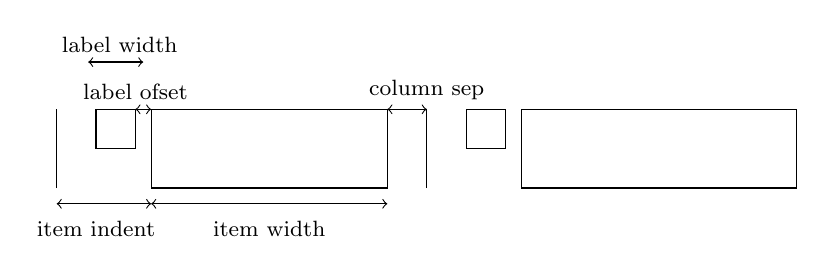
\begin{tikzpicture}
\draw(0,0)--(0,1);
\draw(-3.5,0) rectangle (-0.5,1);
\draw(0.5,0.5) rectangle (1,1);
\draw(1.2,0) rectangle (4.7,1);
\draw(-4.7,0)--(-4.7,1);
\draw(-3.7,0.5) rectangle (-4.2,1);
\draw[<->](0,1)--(-0.5,1);
\draw[<->](-3.5,1)--(-3.7,1);
\draw[<->](-4.7,-0.2)--(-3.5,-0.2);
\draw[<->](-3.5,-0.2)--(-0.5,-0.2);
\draw[<->](-3.6,1.6)--(-4.3,1.6);
\node[above] at (-3.7,1){\footnotesize label ofset};
\node[above] at (0,1){\footnotesize column sep};
\node[below] at (-4.2,-0.3){\footnotesize item indent};
\node[below] at (-2,-0.3){\footnotesize item width};
\node[above] at (-3.9,1.6){\footnotesize label width};
    \end{tikzpicture}
}
\caption{A visual representation of the used lengths.}
\end{figure}

the label will align with the textblock above (if label-align = \{left\} is set). Please see fgure 1
for a sketch of the available lengths and how they are set.

column-sep = {<dim>} \hfill Default: 0pt

A horizontal length that is inserted between columns ot items.
label-align = left $|right|$ center Default: left

Determine show the labels are aligned with in the label-box whose width is set with label-width .
before-skip = \{<skip>\} \hfill Default: 0pt

Sets the skip before the list.
after-skip = \{<skip>\} \hfill Default: 0pt
Sets the skip after the list.
after-item-skip = \{<skip>\} \hfill  Default: 1ex plus 1ex minus 1ex

This vertical skip is inserted between rows of items.

resume = true$|$false \hfill Default: false

The enumeration will resume from a previous tasks environment. In order to use this option
properly you shouldn’t mix diferent tasks environments that both count their items.
start =\{<integer>\} \hfill Default: 1

Set the starting value with which the list starts counting.

counter = \{<counter>\} Default: task

The counter to be used to count the items.
debug = true$|$false Default: false

If set to true \verb|\|\textcolor{Tasks}{fboxsep} is set to 0pt inside the tasks environment and \verb|\|\textcolor{Tasks}{fbox} is used to draw a
frame around the label boxes and the item boxes.

Now the same list as above but with three columns and a diferent label:

\begin{tcolorbox}[collower=black,colframe=Tasks,colback=white]
    \begin{lstlisting}
\begin{tasks}[label=(\roman * ),label-width=4ex](2)
\task \Sample
\task \sample
\task \sample
\task \Sample
\task \sample
\end{tasks}
\end{lstlisting}
        \tcblower
        \settasks{debug}
        \begin{tasks}[
        label=(),
        label-width=4ex
        ](2)
            \task \Sample
            \task \sample
            \task \sample
            \task \Sample
    \end{tasks}
           \end{tcolorbox}

Let's use it inside a question, i.e., inside xsim’s exercise environment [Nie20]:

\begin{tcolorbox}[collower=black,colframe=Tasks,colback=white]
    \begin{lstlisting}
% since settings are local the following ones will be lost
% outside this example;
\settasks{
label = \theexercise.\arabic * ,
item-indent = 2em ,
label-width = 2em ,
label-offset = 0pt
}
\begin{exercise}
I have these two tasks for you. Shall we begin?
\begin{tasks}(2)
\task The first task: easy!
\task The second task: even more so!
\end{tasks}
\end{exercise}
\begin{solution}[print]
Now, let's see\ldots\ ah, yes:
\begin{tasks}
\task This is the first solution. Told you it was easy.
\task This is the second solution. And of course you knew that!
\end{tasks}
\end{solution}
\end{lstlisting}
        \tcblower
% since settings are local the following ones will be lost
% outside this example;
\settasks{
   %label = \theexercise.\arabic * ,
    item-indent = 2em ,
    label-width = 2em ,
    label-offset = 0pt
    }
    I have these two tasks for you. Shall we begin?
    \begin{tasks}[style=enumerate](2)
    \task The first task: easy!
    \task The second task: even more so!
    \end{tasks}

    Now, let's see\ldots\ ah, yes:
    \begin{tasks}[style=enumerate]
    \task This is the first solution. Told you it was easy.
    \task This is the second solution. And of course you knew that!
    \end{tasks}
           \end{tcolorbox}

Finally let’s see what the debug option does (you could see it already on page 6):

\begin{tcolorbox}[collower=black,colframe=Tasks,colback=white]
    \begin{lstlisting}
\settasks{debug}
\begin{tasks}(2)
\task \Sample
\task \Sample
\end{tasks}
\end{lstlisting}
        \tcblower
        \settasks{debug}
        \begin{tasks}(2)
        \task \Sample
        \task \Sample
        \end{tasks}
           \end{tcolorbox}

\section{Available Instances}

There are currently three additional instances for the tasks object available:

{\bfseries itemize} uses \verb|\|\textcolor{Tasks}{labelitemi} as labels.

{\bfseries enumerate} enumerates the items with 1., 2., ...

\begin{tcolorbox}[collower=black,colframe=Tasks,colback=white]
    \begin{lstlisting}
\begin{tasks}[style=itemize](2)
\task that's just how\ldots
\task \ldots we expected
\end{tasks}
\begin{tasks}[style=enumerate](2)
\task that's just how\ldots
\task \ldots we expected
\end{tasks}
\end{lstlisting}
        \tcblower
        \begin{tasks}[style=itemize](2)
            \task that's just how\ldots
            \task \ldots we expected
            \end{tasks}
            \begin{tasks}[style=multiplechoice](2)
            \task that's just how\ldots
            \task \ldots we expected
            \end{tasks}
           \end{tcolorbox}

\section{Custom Labels}

If you want to change a single label inside a list, you can use the optional argument of \verb|\|\textcolor{Tasks}{task}.

This will temporarily overwrite the default label.

\begin{tcolorbox}[collower=black,colframe=Tasks,colback=white]
    \begin{lstlisting}
\begin{tasks}[style=itemize](2)
\task that's just how\ldots
\task[+] \ldots we expected
\task that's just how\ldots
\task \ldots we expected
\end{tasks}
\end{lstlisting}
        \tcblower
        \begin{tasks}[style=itemize](2)
            \task that's just how\ldots
            \task[+] \ldots we expected
            \task that's just how\ldots
            \task \ldots we expected
            \end{tasks}
           \end{tcolorbox}

You’ve already seen examples for the label option.

label = {<code>} Default: \verb|\|\textcolor{Tasks}{alph *} )

It can be used to set the label for a list. A * inside is always replaced by the current counter
name inside braces. It can contain formatting instructions like \verb|\|\textcolor{Tasks}{bfseries} but it can be cleaner
to use

label-format = {<code>}\hfill (initially empty)

instead. This is especially true since the label also sets \verb|\|\textcolor{Tasks}{the<counter>} where you usually don’t
want to have formatting instructions. Another way to deal with this issue is the option

ref = {<code>}\hfill (initially empty)

which sets \verb|\|\textcolor{Tasks}{the hcounteri} ( \verb|\|\textcolor{Tasks}{thetask} in the default setting).

\begin{tcolorbox}[collower=black,colframe=Tasks,colback=white]
    \begin{lstlisting}
\begin{tasks}[label=\arabic * .,ref=\arabic * ]
\task first item
\task second item \label{foo}
\end{tasks} See item~\ref{foo} without dot.
\end{lstlisting}
        \tcblower
        \begin{tasks}[
            %label=\arabic * .,
           % ref=\
            %arabic *
            ]
            \task first item
            \task second item \label{foo}
            \end{tasks}
            See item~\ref{foo} without dot.
           \end{tcolorbox}

Two additional commands are defned which in some circumstances might prove useful:

\verb|\|\textcolor{Tasks}{tasksifmeasuringTF\{<true>\}\{<false>\}}

This command used inside a label checks if the label is typeset for measuring its width or if it is
typeset ``for real''. There are also the variants \verb|\|\textcolor{Tasks}{tasksifmeasuringT} and \verb|\|\textcolor{Tasks}{tasksifmeasuringF}.

\verb|\|\textcolor{Tasks}{tasklabel}

New Holds the current label text.

\section{New tasks-like Environments}

It is possible to add custom environments that work like the tasks environment.

\verb|\|\textcolor{Tasks}{NewTasksEnvironment[<options>]\{<name>\}[<separator>](<cols>)}

\verb|\|\textcolor{Tasks}{Defneenvironment <name> thatuses <eparator> tointroduceanewitem}.

\verb|\|\textcolor{Tasks}{Defaultfor <separator>}

is \verb|\|\textcolor{Tasks}{task}, default for <cols> is 1 . The <options> are the ones described in section 4.

\verb|\|\textcolor{Tasks}{RenewTasksEnvironment[<options>]\{<name>\}[<separator>](<cols>)}

Renew environment previously defned with \verb|\|\textcolor{Tasks}{NewTasksEnvironment}.

The tasks environment is defned as follows:

\begin{tcolorbox}[collower=black,colframe=Tasks,colback=white]
    \begin{lstlisting}
    \NewTasksEnvironment{tasks}
    \end{lstlisting}
\end{tcolorbox}

The separator does not have to be a control sequence:

\begin{tcolorbox}[collower=black,colframe=Tasks,colback=white]
    \begin{lstlisting}
% preamble:
% \usepackage{fontawesome}
\NewTasksEnvironment[label=\faThumbsOUp,label-width=15pt]{done}[ * ]
\begin{done}
* First task
* Second task
\end{done}
\end{lstlisting}
        \tcblower
        %\NewTasks[style=\footnotesize\leftthumbsup,label-width=1.3em]{done}[ * ]
\begin{tasks}(2)
\task[$\clubsuit$] First task
\task[$\spadesuit $] Second task
\task[$\surd $] First task
\task[$\heartsuit $] Second task
\end{tasks}
\end{tcolorbox}

Although this might seem handy or even nice I strongly advice against using something
diferent than a command sequence. Remember that the items will be split at every occurrence
of the separator. So in order to use the separator (here for example for a starred variant of a
command) within an item it has to be hidden in braces. This is avoided of you use a command
sequence which even doesn’t have to be defned.

Please also keep in mind that the separator still has an optional star argument (see 4), an
optional bang argument and the standard optional argument. Using * will prevent the optional
star argument.

\begin{tcolorbox}[collower=black,colframe=Tasks,colback=white]
    \begin{lstlisting}
% preamble:
% \usepackage{fontawesome}
\NewTasksEnvironment[label=\faThumbsOUp,label-width=15pt]{done}[ * ]
\begin{done}(3)
* First task
* Second task
* ! Third task spanning the full width available
* Fourth task
\end{done}
\end{lstlisting}
        \tcblower
        %\NewTasksEnvironment[label=\faThumbsOUp,label-width=15pt]{done}[ * ]
\begin{tasks}(2)
\task[$\nabla $] First task
\task[>>>>] Second task
\end{tasks}
           \end{tcolorbox}


\section{Styling tasks}

TASK uses xtemplate to declare additional instances for the lists.

\subsection{The tasks Object}

The object that’s defned by tasks is the `tasks' object. This time there are four instances
available for the one template (again `default') that was defned.

\subsubsection{Available Options}

This section only lists the options that can be used when defning an instance of the `defaul'
template. The following subsections will give some examples of their usage.

\begin{tcolorbox}[collower=black,colframe=Tasks,colback=white]
    \begin{lstlisting}
\DeclareTemplateInterface{tasks}{default}{3}{
% option : type = default
label : tokenlist = \alph * ) ,
indent : length = 2.5em ,
label-format : tokenlist ,
label-width : length = 1em ,
label-offset : length = .3333em ,
after-item-skip : skip = 1ex plus 1ex minus 1ex
}
\end{lstlisting}
    \end{tcolorbox}

\subsubsection{Predefned Instances}

This is rather brief this time:

    \begin{tcolorbox}[collower=black,colframe=Tasks,colback=white]
        \begin{lstlisting}
% alphabetize: a) b) c)
\DeclareInstance{tasks}{alphabetize}{default}{}
% itemize
\DeclareInstance {tasks} {itemize} {default}{
label-width = 1.125em ,
label = \labelitemi}  % enumerate:
\DeclareInstance {tasks} {enumerate} {default}
{label = \arabic * . }
    \end{lstlisting}
        \end{tcolorbox}

\begin{thebibliography}{9}

\bibitem{1} Javier Bezos. enumitem. Version 3.9. June 20, 2019. url: https://ctan.org/pkg/enumitem.

\bibitem{2} The \LaTeX{}3 Project Team. l3kernel. Sept. 19, 2019.
url: https://www.ctan.org/pkg/ l3kernel/.

\bibitem{3} Clemens Niederberger. exsheets. Version 0.21k. Sept. 30, 2019.
url: https://ctan. org/pkg/exsheets.

\bibitem{4} Clemens Niederberger. xsim. Version 0.19a. Mar. 19, 2020.
url: https://ctan.org/pkg/xsim.

\bibitem{5} Will Robertson. environ. Version 0.3. May 4, 2014.
url: https://ctan.org/pkg/environ .

\end{thebibliography}
\end{document}